\documentclass[a4paper]{article}
\usepackage{multicol}
\setlength{\columnsep}{3cm}
\usepackage{parskip}
\usepackage{changepage}
\usepackage[T1]{fontenc}
\usepackage{amsmath}
\usepackage{listings}
\usepackage{amsthm}
\usepackage{amssymb}
\usepackage{float}
\usepackage[utf8]{inputenc}
\usepackage{graphicx}
\usepackage[italian]{babel}
\usepackage{thmtools}
\newtheorem*{theorem}{Teorema}
\newtheorem*{definition}{Definizione}
\newtheorem{example}{Example}
\newenvironment{dimostrazione}{\textit{Dimostrazione}:\begin{adjustwidth}{2cm}{}}{\end{adjustwidth}}

\begin{document}

\author{Lorenzo Dentis, lorenzo.dentis@edu.unito.it}
\title{Risposte AlgComp}
\maketitle

\section{Brute-force e certificazione}
\subsection{A.1}
Posto un array $V$ di $n$ elementi individuo due indici, $i$ e $j$.\\L'idea è di mantenere gli elementi $[0 ... j-1]$ fissi ed andare a generare tutte le permutazioni dei restanti elementi $[j ... n-1]$grazie all'indice $i$.

Ad ogni incremento dell'indice $i$ segue una sequenza di chiamate ricorsive che hanno lo scopo di effettuare uno swap fra l'elemto di indice $i$ e l'elemento di indice $j$ e poi incrementare $j$ scendendo nell'albero della ricorsione fino alla condizione $j=i$, quando $i$ viene di nuovo incrementato.Intuitivamente $j$ indica la profondità della ricorsione, $i$ indica l'ampiezza.
\begin{itemize}
	\item \textbf{Punto 1}:L'algoritmo è completo in quanto genera $n!$ permutazioni, ed è corretto in quanto sono tutte distinte.\\Le permutazioni generate sono esattamente $n!$ in quanto alla "radice" dell'albero avrò $n$ chiamate ricorsive (con $i = 0, i=1, ... i= n-2, i=n-1$ ).Invece al livello di profondità $j$ i primi $j$ elementi del vettore risulteranno fissi ed avrò solo $n-1-j$ chiamate ricorsive.\\Considerando che il valore di $j$ viene incrementato di una unità ad ogni "livello" di ricorsione fino all' $n-(n-1)$esimo livello ottengo questa semplice equazione: \begin{center}$calls = n * (n-1) * ...(j-1$volte$)... * 1$\end{center}Che non è altro che $n!$


		Le permutazioni sono tutte distinte perchè $i$ e $j$ non assumono mai due volte lo stesso valore, posto che ogni elemento del vettore sia distinto.Di conseguenza lo "swap" avverrà sempre tra due elementi differenti ad ogni chiamata ricorsiva impedendo la costruzioni di due permutazioni uguali.
	\item \textbf{Punto 2}:Un algoritmo che generi \textit{tutti i sottoinsiemi di elementi} può essere realizzato
\end{itemize}
\subsection{A.2}
Definizione formale di una permutazione (definizione ricorsiva):
\begin{figure*}[!ht]
\centering
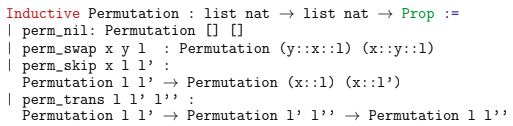
\includegraphics[width=0.7\textwidth]{./img/permutazione_ricorsiva.png}
\caption{Definizione ricorsiva di una permutazione} \label{FIG:recursive_permutation1}
\end{figure*}
\begin{itemize}
	\item perm\_nil: [ ] è permutazione di [ ] (lista vuota è permutazione di se stessa)
	\item perm\_swap: $\forall x,y \in Elements$ e $\forall l \in Lists$ $[y::x::l]$ e $[x::y::l]$ sono una permutazione dell'altra
	\item perm\_skip: dato $x \in Elements$, se $l \in Lists$ è permutazione di $l' \in Lists$ $\Rightarrow [x::l]$ è permutazione di $[x::l']$
	\item perm\_trans: date $l, l', l'' \in Lists$ se $l$ permutazione di $l'$ e $l'$ permutazione di $l'' \Rightarrow l$ è permutazione di $l''$ 
\end{itemize}
\begin{theorem}[Riflessività] $\forall l \in Lists$ Permutation $l$ $l$\end{theorem}
\textit{Dimostrazione}:
\begin{adjustwidth}{2cm}{}
	\textit{caso base}: $l$ = [ ], vale per definizione grazie a perm\_nil\\
	\textit{caso induttivo}: $l = [h::t]$ con $h \in Lists$ e $t \in ELements$.\\
	Grazie all'ipotesi induttiva si può affermare \textit{Permutation} $t$ $t$ e quindi per perm\_skip \textit{Permutation} $[h::t]$ $[h::t]$. Dato che $l = [h::t]$ abbiamo che \textit{Permutation} $l$ $l$.
\end{adjustwidth}
\begin{theorem}[Simmetria] $\forall l,l' \in Lists$, Permutation $l$ $l'$ $\Rightarrow $ Permutation $l$ $l'$\end{theorem}
\begin{dimostrazione}
	DA FAR
\end{dimostrazione}
\subsection{A.3}
Dimostrare che è algoritmo che genera permutazioni di una lista di elementi è completo significa dimostrare che genera $n!$ permutazioni, con $n$ pari al numero di elementi. Formalmente:
\begin{theorem}[Completezza] $\forall l \in Lists$, $len($\textit{permutation} $l) = len(l)!$\end{theorem}
\begin{dimostrazione}
	\textit{caso base}: $l$ = [ ]\\
	In questo caso $len(l)! = 0! = 1$.\\
	Allo stesso modo $len(permutation)$ [ ] $= len($[ [ ] ]$) = 1$.\\
	Quindi $len($\textit{permutation} $l) = len(l)!$
	
	\textit{Caso induttivo}: $l = h::t$, quindi l'enunciato da dimostrare è $len($\textit{permutation} $[h::t]) = len([h::t])!$\\
	$len(h::t) = 1 + len(t)$\\
	Quindi $len(distribute$ $a$ $[h::t]) = 2 + len(t)$ che per il Lemma distribute\_lenght diventa $len((a::t)::distribute$ $a$ $t) = 2 + len(t)$
	INSERIRE FOTO LEMMA DISTRIBUTE
\end{dimostrazione}

\section{Backtrack}
\section{Branch&Bound}
\end{document}
